\section{Radioastronomie}
\sectionauthor{Constantin Burmeister, (Ole Fleck)}

Radioastronomie dient der Beobachtung von astrophysikalischen Prozessen, die Radiowellen, also Wellen langer Wellenlänge, aussenden. Um hohe Auflösungen zu erreichen, werden Radiointerferometer verwendet, welche Signale mehrerer Antennen so zusammenfügen, als würde es sich um eine Antenne handeln.

Allgemein ist der minimal auflösbare Bildwinkel $\delta\theta$ eines Teleskops abhängig von der Wellenlänge $\lambda$, des beobachteten Lichts, und dem Spiegeldurchmesser $D$ des Teleskops mit \begin{eqnarray} \label{k4.2.radioformel}
\delta\theta\approx1.22\frac{\lambda}{D}.
\end{eqnarray}
Da die Radioastronomie große Wellenlängen verwendet, sind hier auch bei Teleskopen mit großen Spiegeldurchmessern von über $100\text{m}$ nur geringe Auflösungen möglich.

\begin{figure}
\centering
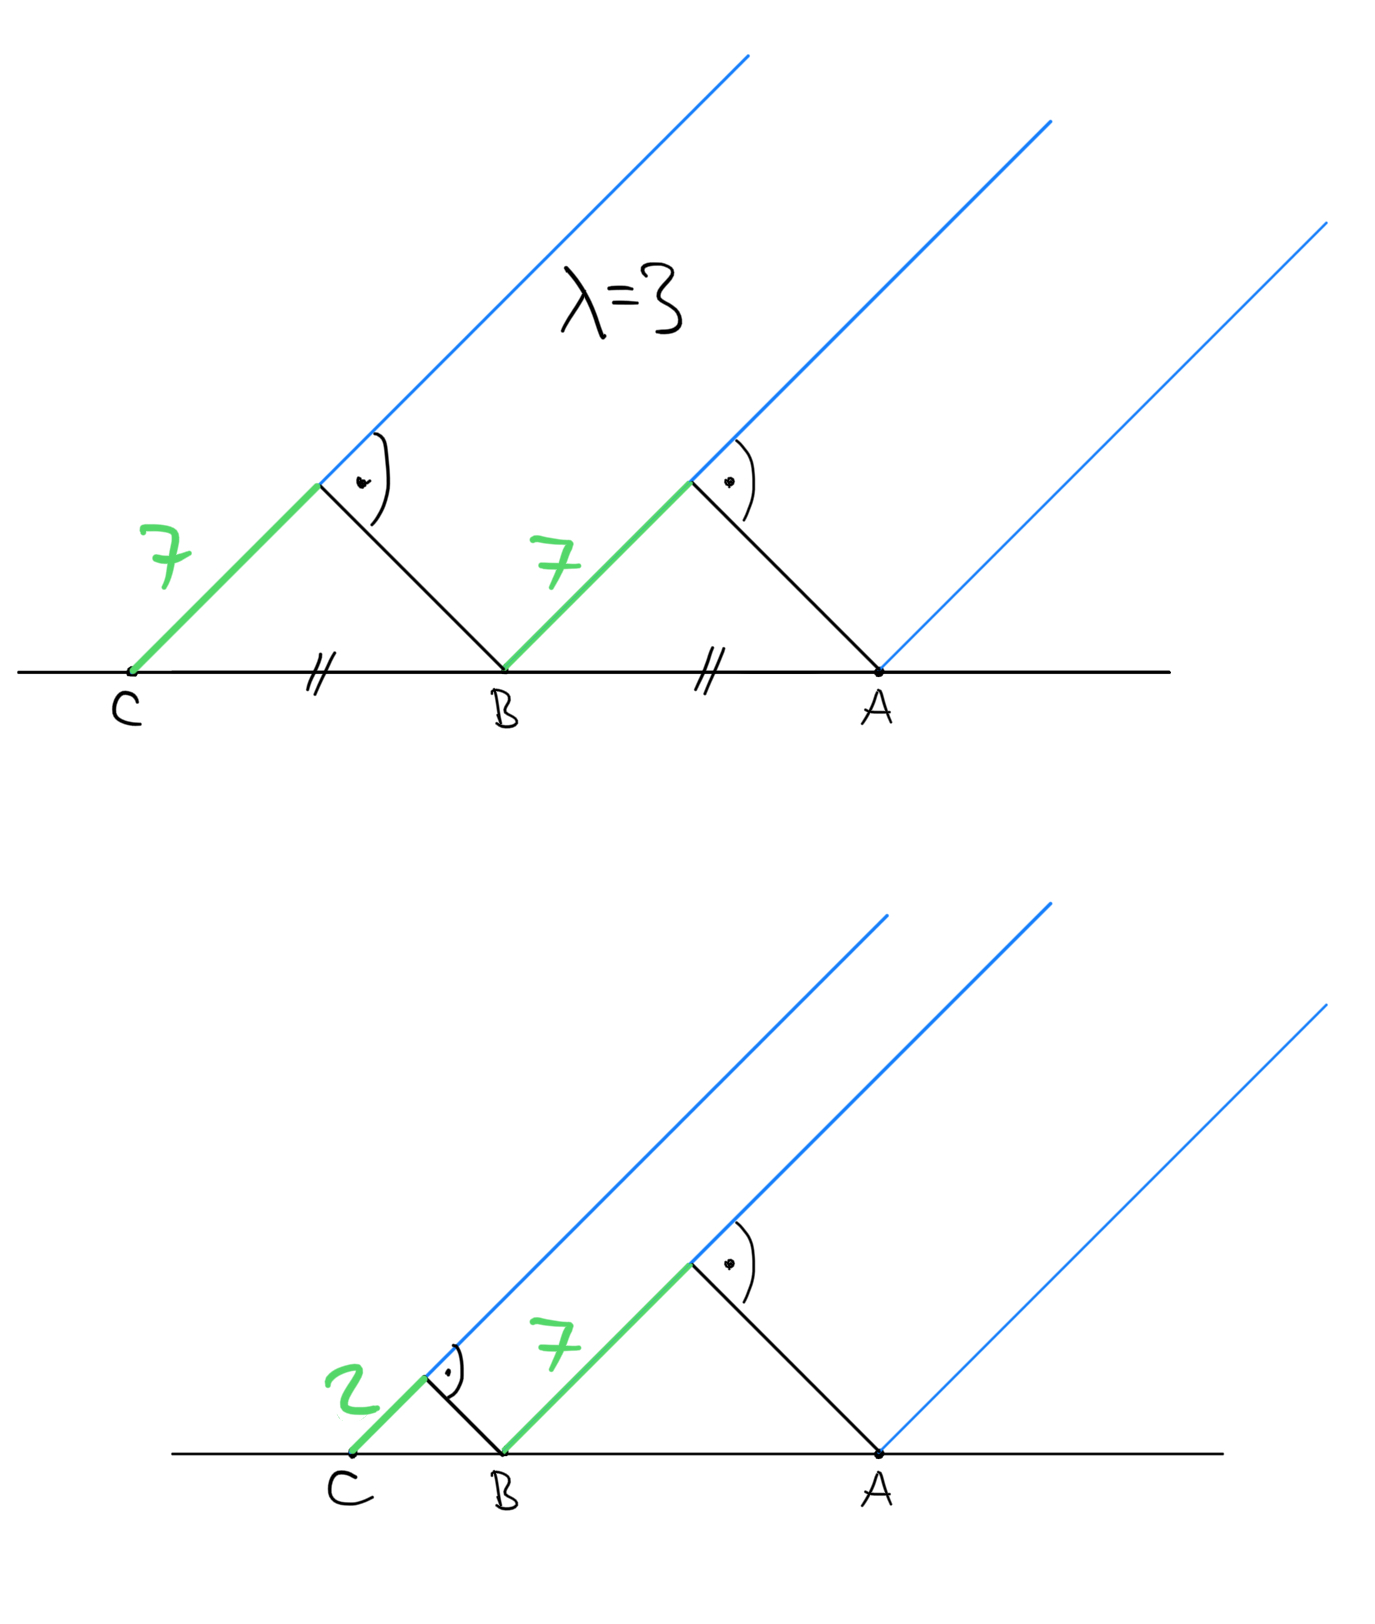
\includegraphics[width=.4\textwidth]{k4.2/baselineunterschied.png}
\caption{Gangdifferenzen von Radiowellen bei Antennenarrays (A,B und C) mit Wellenlänge $\lambda = 3$}
\label{bild-baselineunterschied}
\end{figure}

Zur Kompensation dieses Problems wurde die Radiointerferometrie entwickelt.
Das Verfahren dient zur Überlagerung von Radiowellen, welche von mehreren Antennen aufgezeichnet wurden, um eine höhere Auflösung zu erzielen als es mit einer einzelnen Antenne möglich wäre.
Das hieraus resultierende Signal ist vergleichbar mit dem Signal, welches von einer Antenne mit dem Spiegeldurchmesser entsprechend des Antennenabstandes erzeugt worden wäre.

Ein Interferometer kann nur die Laufzeitdifferenz zwischen Wellen bestimmen, da die einzelnen Wellenberge nicht unterschieden werden können. So können, wie im Beispiel  \cref{bild-baselineunterschied}, bei gleichen Abständen zwischen den Teleskopen A,B und C nicht zwischen den Gangdifferenzen modulo der Wellenlänge, welche im Beispiel $\lambda = 3$ beträgt, unterschieden werden. In diesem Beispiel ist aus den Messwerten nicht ersichtlich, ob es sich tatsächlich um $2\cdot \lambda +1 = 7$ Gangunterschied handelt, sondern jedes $n\in \mathbb{N}$ in $n\cdot\lambda+1$ ist möglich. Die Differenz könnte also immer auch um vielfache von 3 Längeneinheiten verschieden sein. Werden Antennen mit unterschiedlichen Abständen verwendet, sinkt die Anzahl der Kombinationen der Gangunterschiede, für welche sich eine solche Gleichung lösen lässt wie im Beispiel. Hier müssen die Ergebnisse der Gleichung für das untere Bild kongruent zu $3\mathrm{mod}\,2$ sein. Daher werden bei Antennengruppen möglichst viele unterschiedliche Abstände verwendet.

Für die Messung des Radiosignals gilt:
\begin{eqnarray}
d_{uv\lambda} =\int\int I(l,m)e^{-2\pi i \frac{1}{\lambda}(lu-mv)dldm}
\end{eqnarray}
Hier bezeichnet $l$ die Nord-Süd-Achse und $m$ die Ost-West-Achse, $\lambda$ bezeichnet die Beobachtungswellenlänge, und $u$ und $v$ ist der Verbindungsvektor zwischen zwei Antennen. Zusätzlich bezeichnet $n_{uv\lambda}$ ein additives Rauschen. Diese Messgleichung hat große Ähnlichkeit zur Fourier-Transformation (siehe \cref{k4.2.fourier}) und kann als nicht-äquidistante Fourier-Transformation interpretiert werden.

Dieses Verfahren wurde beispielsweise auch beim \emph{Event Horizon Telescope} verwendet. Das \emph{Event Horizon Telescope} besteht aus einer Verschaltung von elf Teleskopen, wobei deren Abstand bis zu $10000\,\text{km}$ beträgt. Mit diesem Teleskop wurde das erste Mal der Schatten eines Schwarzen Lochs beobachtet.

Radiointerferometrie ist also ein essenzieller Bestandteil der Astronomie. Das Verfahren er\-möglicht die Ursprungsbestimmung eines Radiosignals von astrophysikalischen Prozessen bei hoher Auflösung.
